\documentclass[../Head/Main.tex]{subfiles}
\begin{document}
\subsubsection{Line detection}
The line detection consists of the methods \texttt{find\_lines()} and \texttt{merge\_lines()}.\\
The method \texttt{find\_lines()} processes the datapoints by using the incremental line extraction algorithm. This algorithm first computes a line model for 2 points by calculating the line parameter described in section \ref{subsubsec:DesignLineDection}. When it recomputes the line model every time an extra point is added. Before recomputing the line model, the line parameters are stored. This means that the algorithm constantly updates the line parameters for the current and previous line model.\par
Due to the fact, that the algorithm constantly updates the line parameters for the current and previous line model, it does not have to recompute the previous line model, when the current line model does not satisfy the line conditions. \par
To test the performance and robustness of the algorithm a  test with several repetitions were conducted. This test in described in appendix (\ref{test:LineDetection}).
\begin{figure}[H]
  \begin{subfigure}[b]{0.3\textwidth}
  	\centering
    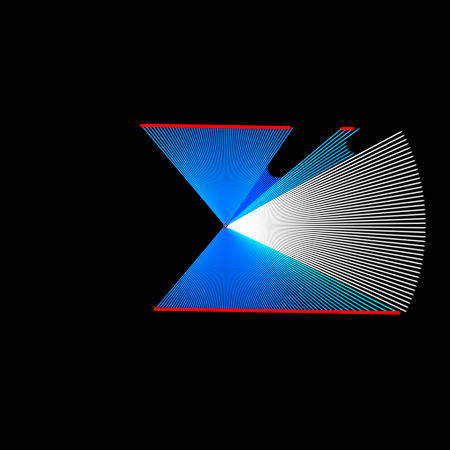
\includegraphics[width=1\textwidth]{Lidar/Test_1_lines}
    \caption{Illustration of data for test 1}
    \label{fig:LineTest1}
  \end{subfigure}
  \hfill
  \begin{subfigure}[b]{0.3\textwidth}
  	\centering
    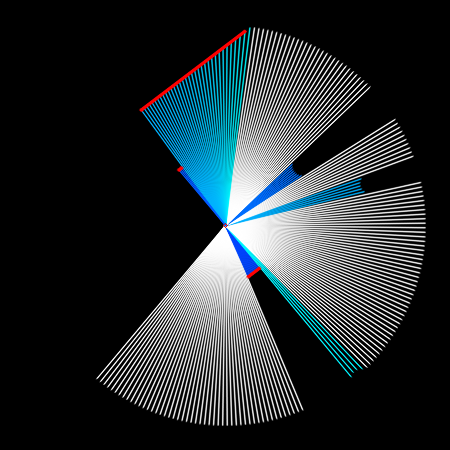
\includegraphics[width=1\textwidth]{Lidar/Test_5_lines}
    \caption{Illustration of data for test 5}
    \label{fig:LineTest5}
  \end{subfigure}
  \hfill
  \begin{subfigure}[b]{0.3\textwidth}
    \centering
    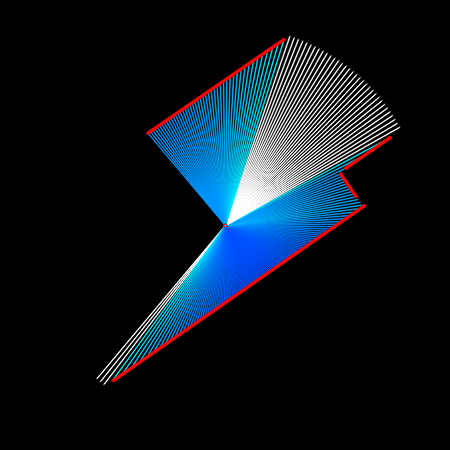
\includegraphics[width=1\textwidth]{Lidar/Test_6_lines}
    \caption{Illustration of data for test 6}
    \label{fig:LineTest6}
  \end{subfigure}
  \caption{Illustration of data for marble detection tests}
  \label{fig:LineTests}
\end{figure}
As mentioned in appendix (\ref{test:LineDetection}), the method \texttt{find\_lines} is robust and has a good performance, since it finds all obstacles such as walls, corners and doorframes. This is also shown in figure (\ref{fig:LineTests}).\par
All the found lines in the area of the sensor range is stored for further processing by the line merging method \texttt{merge\_lines()}.
The method \texttt{merge\_lines()} takes parameters from found lines, and check for two merging conditions The first condition is the angle between two found lines. This condition is called \texttt{threshold} and is defined to 0.1. The second condition is the area the marble provides shade. The algorithm does that by checking the difference in the angle from the end/start point of an found line to the closest line that strikes the marble. This condition is called \texttt{thresholdAlpha} and is defined to 0.5. The second condition prevents that two lines, that corresponds to doorframes, is merged. This means that the lines are not merged, if a marble is in front of a doorway to another room.\par
To test the performance and robustness of the algorithm a  test with several repetitions were conducted. This test in described in appendix (\ref{test:LineDetection}).
\begin{figure}[H]
  \begin{subfigure}[b]{0.5\textwidth}
  	\centering
    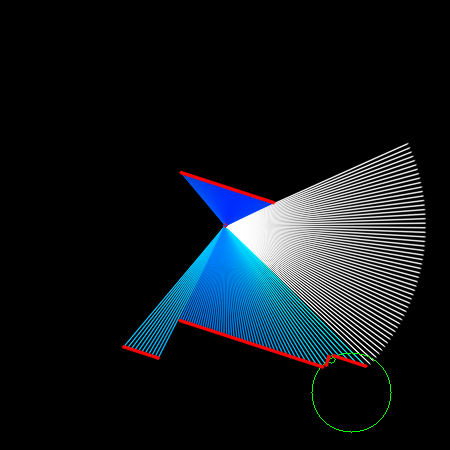
\includegraphics[width=0.6\textwidth]{Lidar/Test_7_lines}
    \caption{Illustration of data for test 7}
    \label{fig:LineTest7}
  \end{subfigure}
  \hfill
  \begin{subfigure}[b]{0.5\textwidth}
  	\centering
    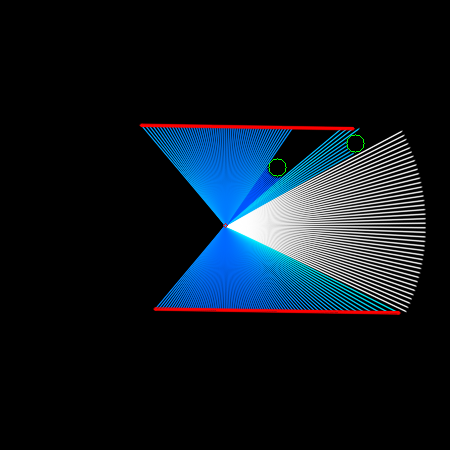
\includegraphics[width=0.6\textwidth]{Lidar/Test_8_lines}
    \caption{Illustration of data for test 8}
    \label{fig:LineTest8}
  \end{subfigure}
  \caption{Illustration of data for marble detection tests}
\end{figure}
As mentioned in appendix (\ref{test:LineDetection}), the line merging method \texttt{merge\_lines()} is robust and has a good performance, since it merges the two lines, which is divided by a marble as shown on figure (\ref{fig:LineTest8}). \par
The method depends on a marble detection method, which is not robust and do not have a good performance, since it detects corners as marbles as shown on figure (\ref{fig:LineTest7}) and detects multiple marbles, when there is only one, as explained in section \ref{subsubsec:Implementation_marble}.
\end{document}